%
% glcd.tex
% Graphical LCD.
%
% LulzBot® TAZ User Manual
%
% Copyright (C) 2015 Aleph Objects, Inc.
%
% This document is licensed under the Creative Commons Attribution 4.0
% International Public License (CC BY-SA 4.0) by Aleph Objects, Inc.
%

The Graphic LCD allows you to print with the LulzBot\textsuperscript{\miniscule{\textregistered}} TAZ 3D printer without needing to have a computer connected or using host software such as Cura. This will allow for more efficient space in the workspace and free up a computer for other tasks.

In the following sections you will find general information on using the Graphic LCD, how to transfer .gcode files to the included SD card, heat up the printer, start a print, and make configuration adjustments.

\section{\texttt{GLCD Controller, Cura or Printrun Host?}}
\label{sec:Graphic LCD, Cura or Printrun Host?}
The Graphical LCD Controller is perfect for normal day to day printing and will be used in the majority of your print jobs. However, in some instances- you will want to use Cura or Printrun instead of the GLCD Controller. A few examples of when you would want to plug the USB cable back in and use Cura:
\begin{itemize}
	\item A number of manual movements are required to perform calibration checks. Because of this it is easier and faster to make the required manual movements within Cura. Calibration checks can be done with the Graphic LCD, but require a number of repetitive menu selections.
	\item Printrun offers a number of extra options for advanced users, including custom gcode input, output display, and pronsole. Pronsole is the command line portion of Printrun that can be used in scripts for automation or controlling a printer through remote access, for example, SSH.
	\item Cura is the preferred printer host software, as the inclusion of quick print profiles, the combination of slicing engine, and printer host communications allows for easy all-in-one use.
\end{itemize}

\section{\texttt{Multiple Connections}}
Because the LulzBot TAZ 3D printer can be controlled by the Graphic LCD and by host software, caution is advised when connecting to the printer through USB as the print can be interrupted when connecting or disconnecting the USB cable. A general rule is: once you have started a print with either the Graphic LCD, Cura, or Printrun, for the rest of the print use only that controller. When printing with the Graphic LCD, never try to connect through USB in the Cura host software; wait until the print is complete, and then connect in Cura.

\section{\texttt{Putting Print Files on the SD Card}}
To print from the Graphic LCD, you will need to transfer .gcode print files onto the SD card. Follow the normal steps, as explained in the Slic3r chapter, to create .gcode print files on your computer. Insert the SD card into your computer using a SD reader slot or USB SD card reader. Open a file browser- / -manager and locate the created .gcode files; drag and drop or paste the .gcode files to the SD card. Once the files have transferred, eject the SD card from your computer and insert it back into the SD card slot on the left side of the Graphic LCD case.

\section{\texttt{Printing With the Graphic LCD}}
\begin{figure}[b]
\centering
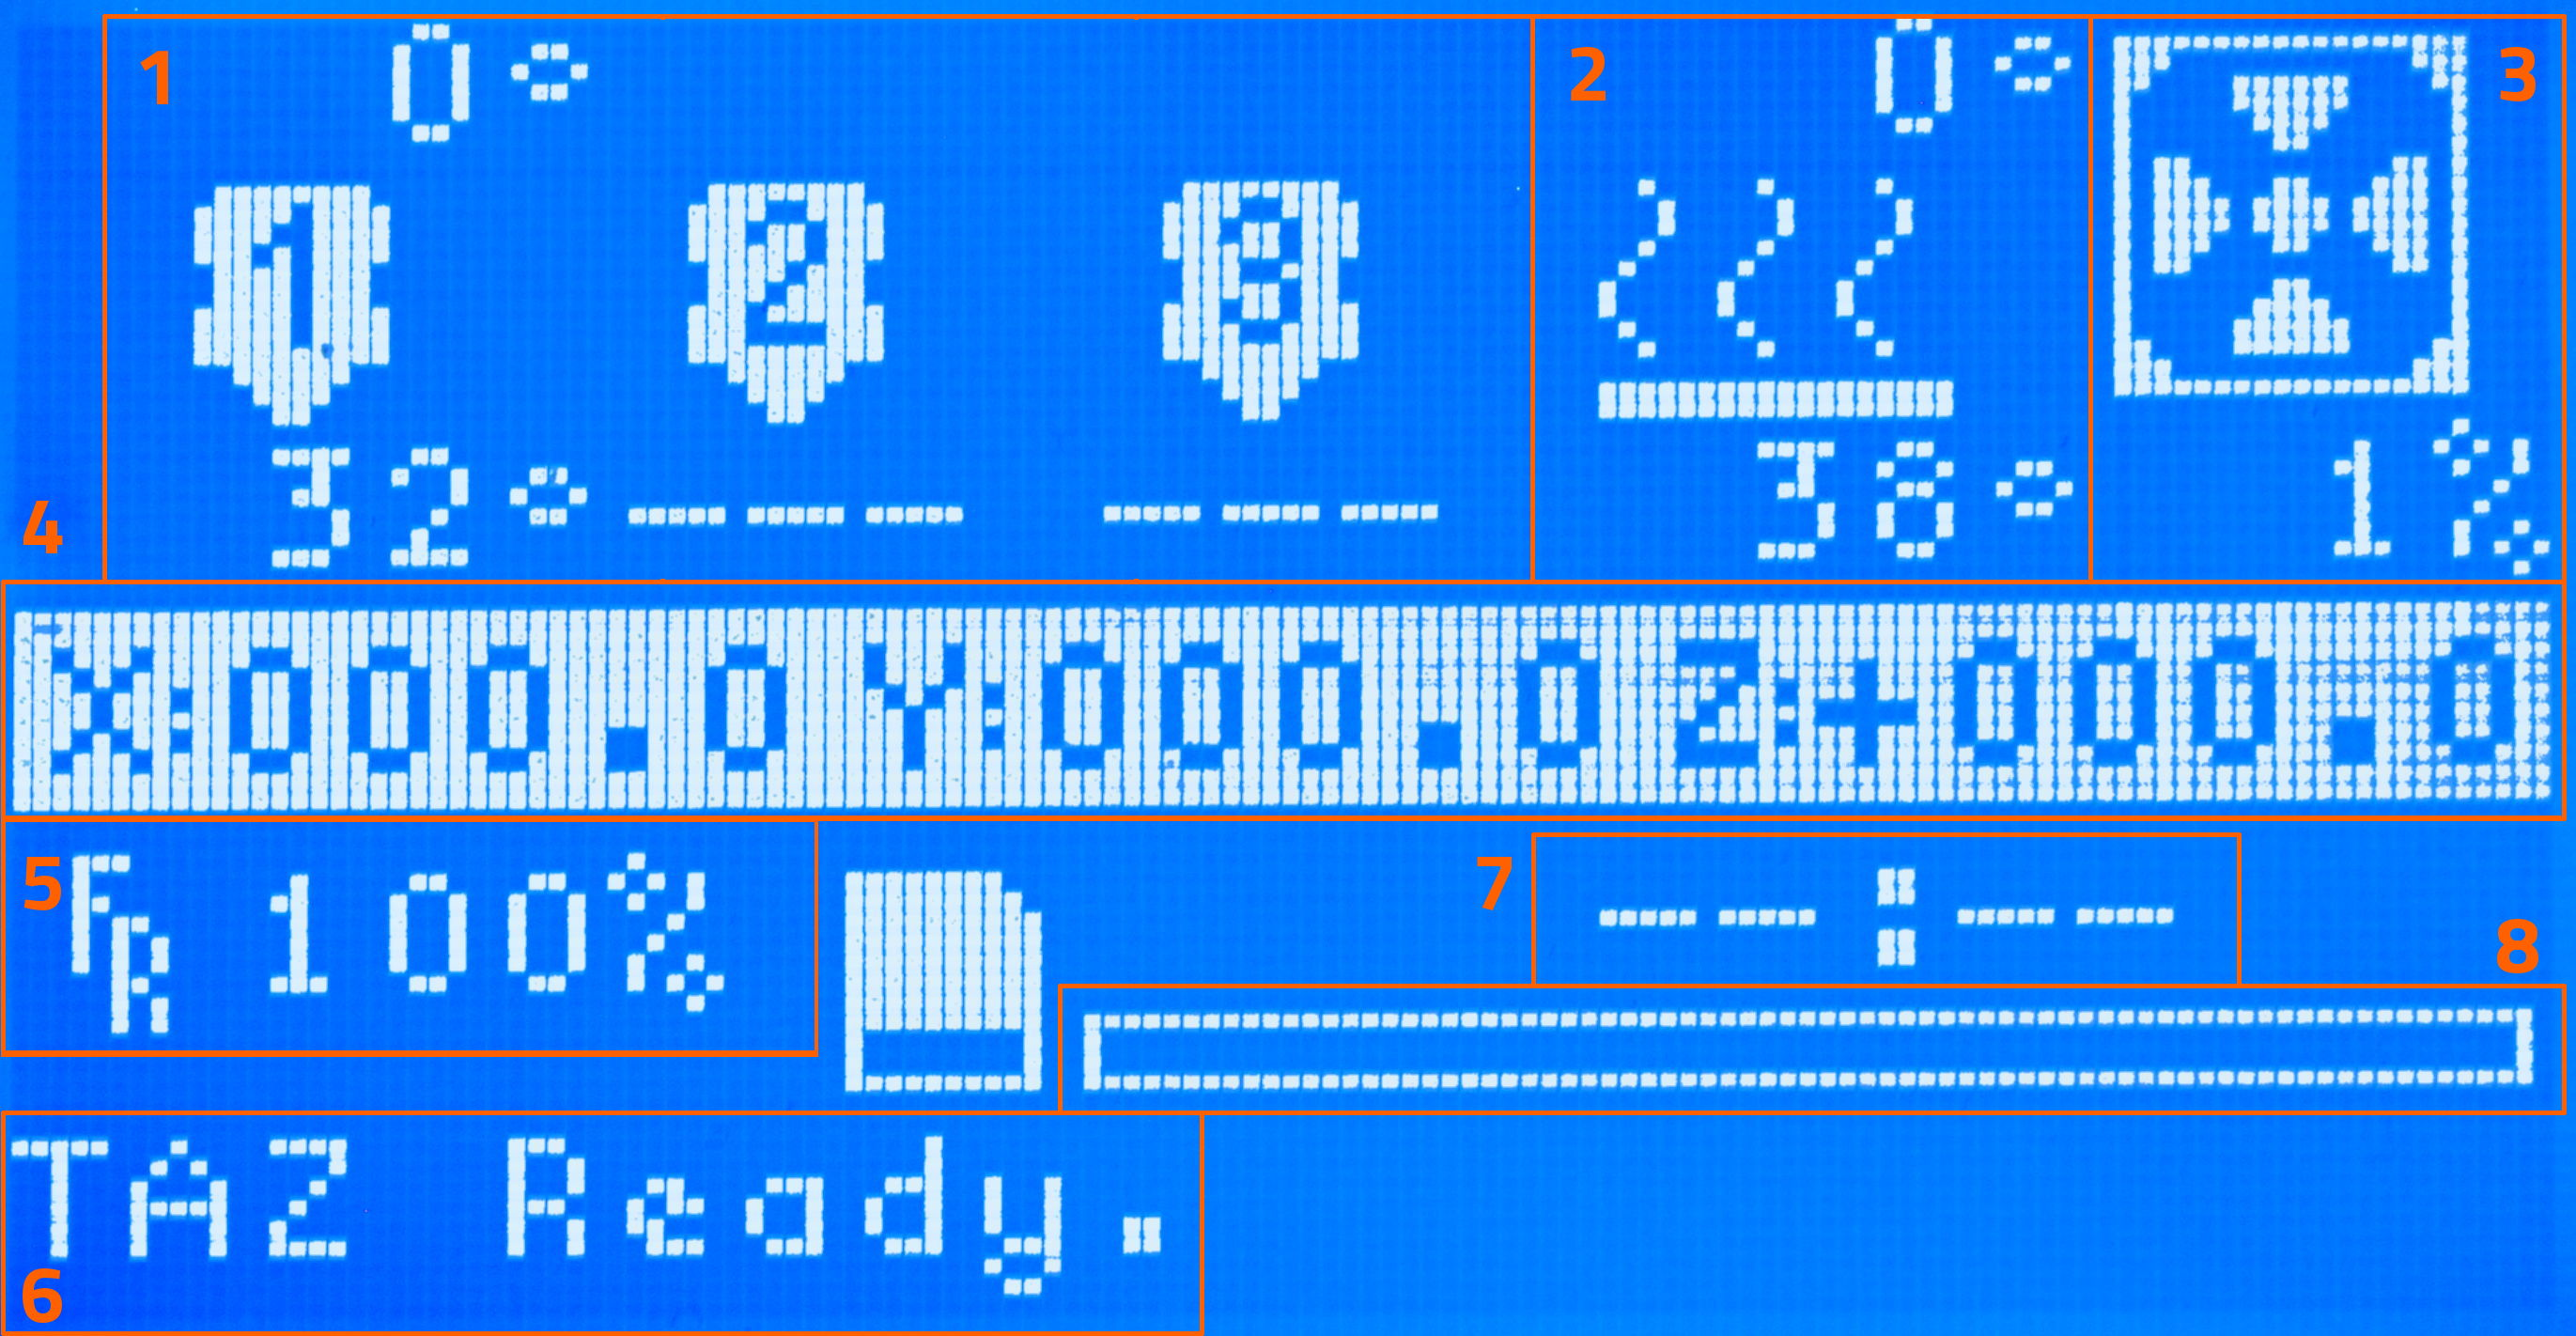
\includegraphics[keepaspectratio=true,angle=0,height=0.4\textheight,width=1.0\textwidth]{LCD_main_screen.jpg}
\caption{GLCD Info Screen}
\label{fig:info_screen}
\end{figure}

\subsection{\texttt{The Graphic LCD Status Screen}}
The GLCD screen will turn on you power up your LulzBot TAZ 3D printer. The start-up screen will display the Status screen (fig. \ref{fig:info_screen}, page \pageref{fig:info_screen}). The Status screen is the default screen for the GLCD, presenting the current status of the printer. There are a number of live statuses shown on the Status screen; these will give you current temperatures, tool head coordinates, print status, and more. The different numbered sections of the status screen are shown in Figure \ref{fig:info_screen} above. Follow the key below for more information on each section.

\begin{enumerate}
\item Hot end temperatures: represents the current temperature (bottom) and set temperature (top) of up to three nozzles. The RAMBo control electronics currently only supports two hot ends.
\item Heat bed temperature: represents the current temperature (bottom) and set temperature (top) of the heat bed.
\item Fan speed: represents the current optional extruder fan speed. The fan is set to off (1\%) by default; the fan is not recommended for ABS. If you print with PLA filament, you will want to use the fan. If cooling is turned on in Cura/Slic3r, this portion of the display will change to reflect the .g-code embedded extruder fan control instructions.
\item Tool head coordinates: represents the current tool head coordinates on the X, Y, and Z axes.
\item Feed rate: represents the current feed rate setting. The feed rate is set to 100\% by default; this matches the speed set in the gcode generation. When on, the status screen selection knob can be turned to increase or decrease the feed rate during the print. Increasing/decreasing the feed rate will increase/decrease the speed of the print.
\item Printer status: lists the current status of the printer including: SD card status, current printing file, or completed print time.
\item Current print time: lists the length of time for the current print job.
\item Progress bar: represents the progress of the current print job. The print is finished when the bar is completely white.
\end{enumerate}


\subsection{\texttt{Using the Selection Knob}}
To navigate through the LCD menu use the selection knob by rotating to scroll through selections and pressing the knob to make a selection. From the main Status screen, press the knob to move into the menu screen (Figure \ref{fig:main_menu}, page \pageref{fig:main_menu}). To move backwards in the menu tree, select the top most menu selection on the current screen. Selections that will move you backwards through the menu tree are noted by an upwards-facing arrow. Note that if the menu is left idle it will automatically move back to the main Status screen.

\begin{figure}[h]
\centering
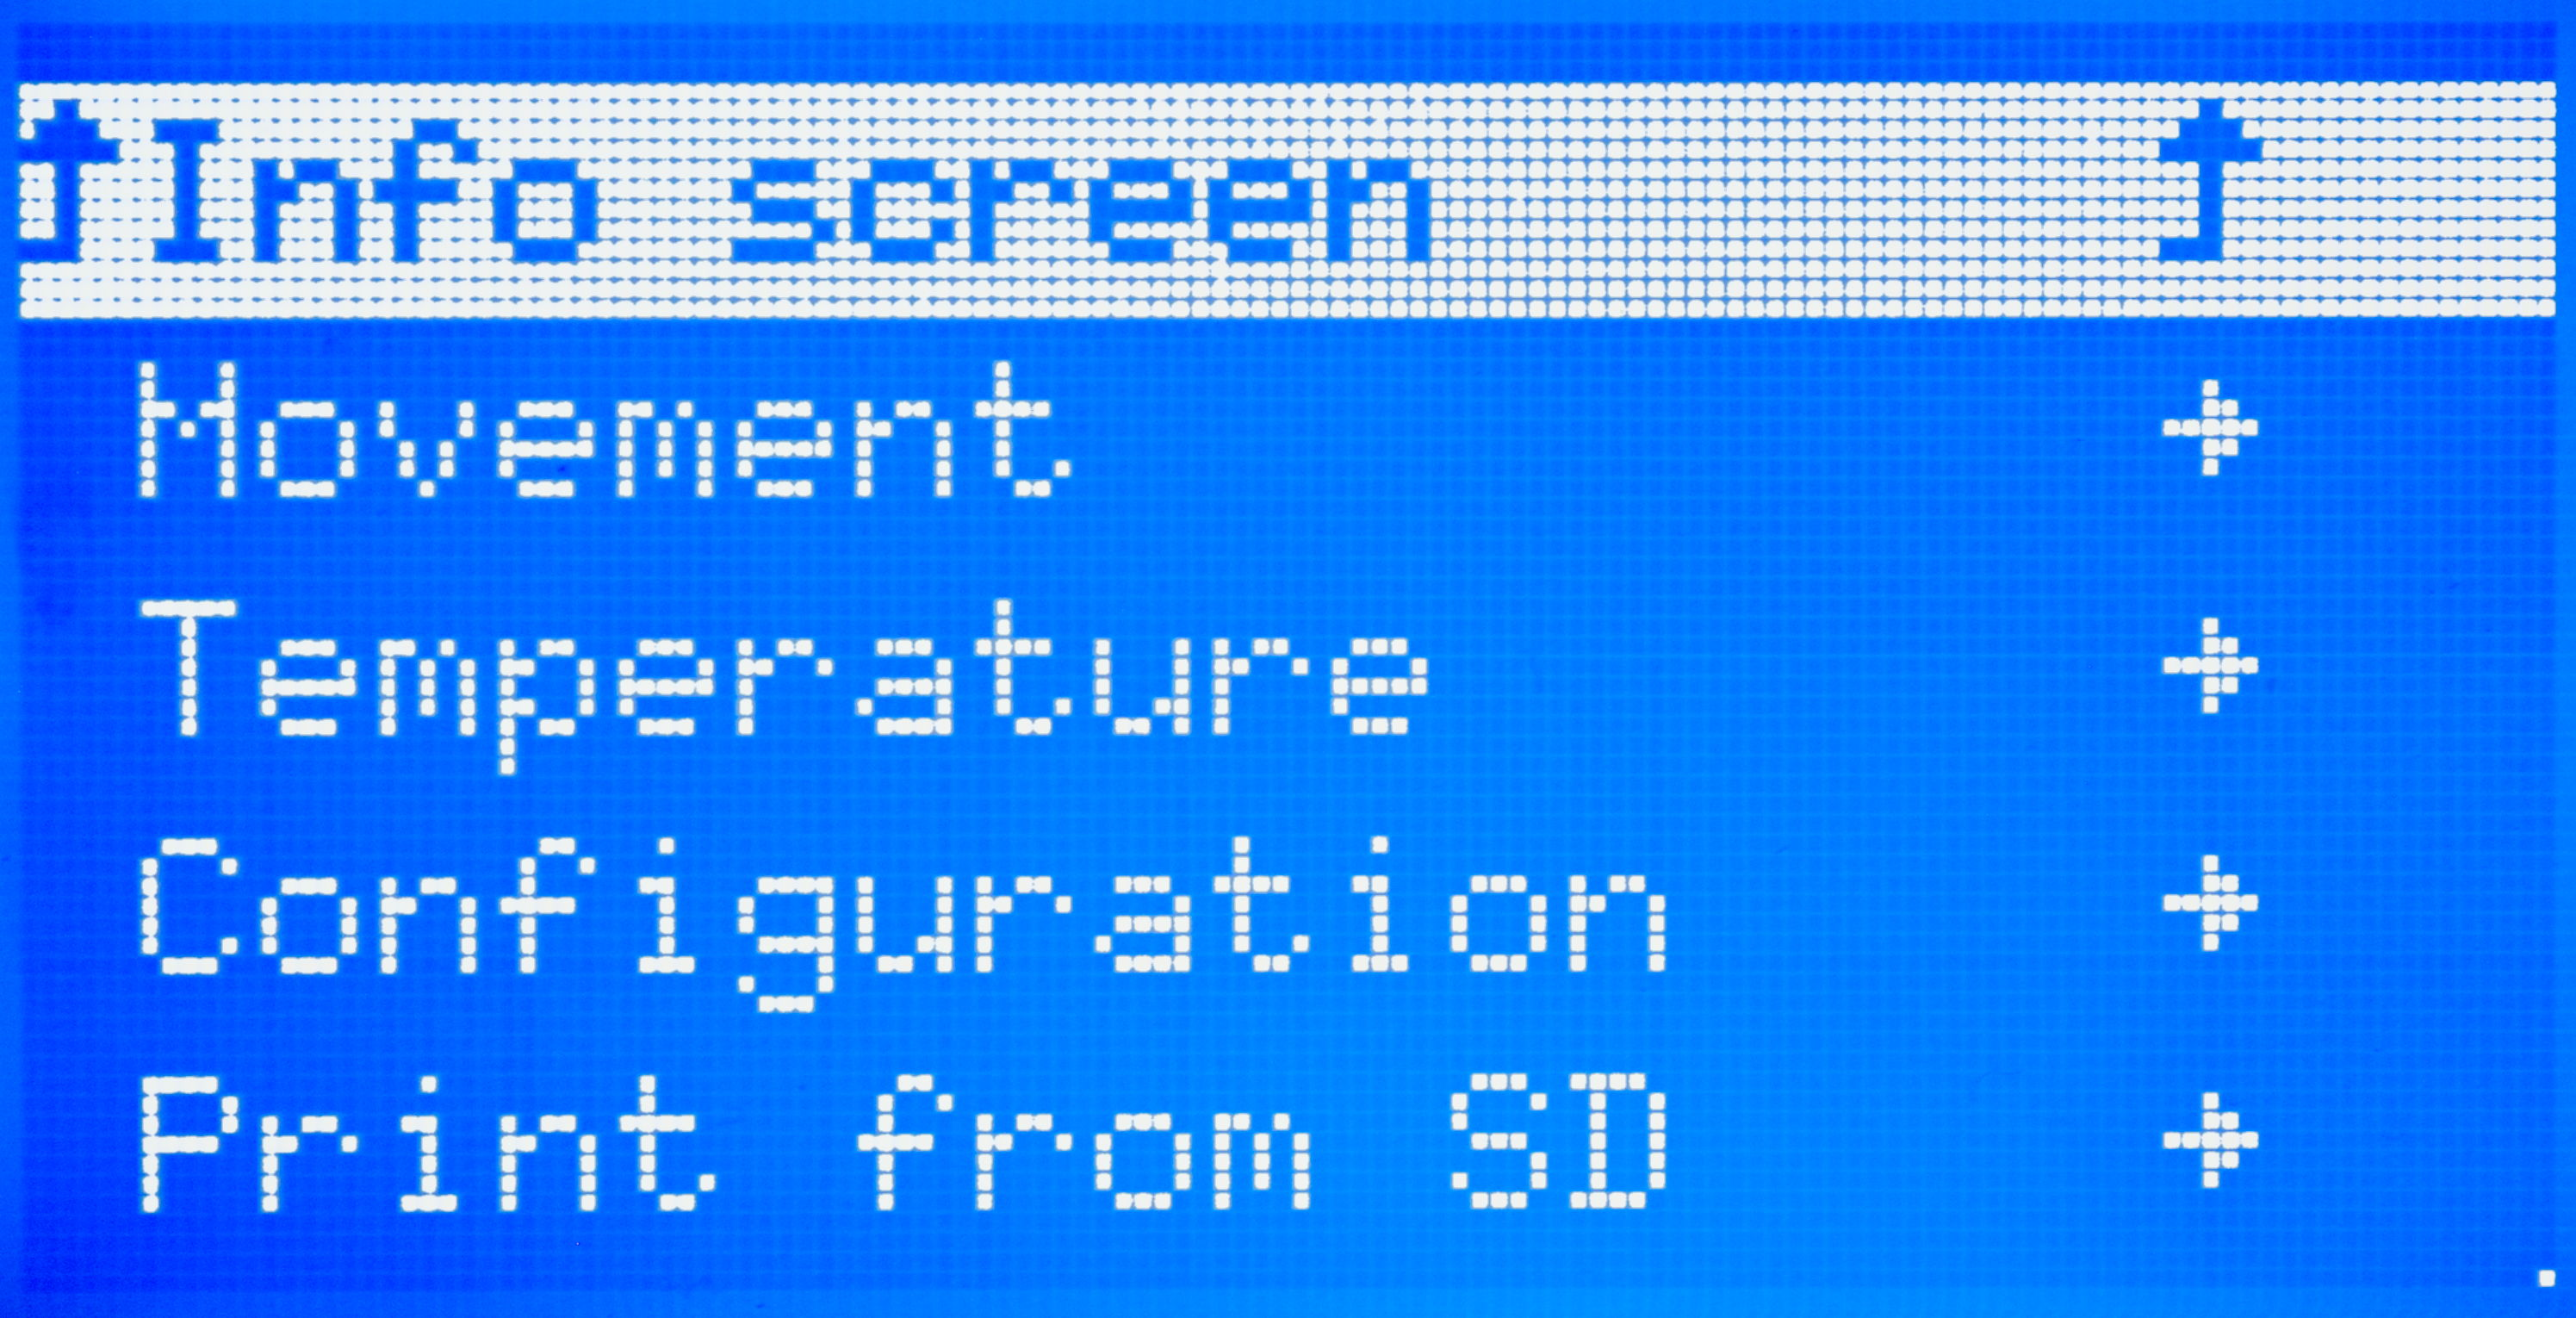
\includegraphics[keepaspectratio=true,angle=0,height=0.4\textheight,width=1.0\textwidth]{LCD_Menu.jpg}
\caption{Main Menu}
\label{fig:main_menu}
\end{figure}

%\subsection{\texttt{Preparing for a Print}}
%Before starting a print you will need to set the hot end and heat bed to the appropriate temperatures for the filament type you are using. To quickly set the printer to preheat, click the selection knob to bring up the menu and select \texttt{Temperature}. Select \texttt{Filament Type} to automatically set the hot end and bed temperature for that specific filament.

%If you need to set the extrusion and/or bed temperature to a setting different than the preheat temperature you can manually set the temperature. To do so, from the main menu navigate through: Temperature \texttt{->} Custom Temp \texttt{->} Nozzle or Bed. Clicking on either of these settings will give you a menu to set and select the desired temperature setting.

\subsection{\texttt{Selecting a File From the SD and Starting a Print}}
Once the SD card has the desired Gcode file loaded onto it, you can begin your first print. From the main menu select the \texttt{Print from SD} option. You will now see a selection of the directories and .gcode files on the SD card. Navigate through the menu to locate the file you would like to print. Select the desired file to begin the print.


\subsection{\texttt{Making Manual Movements With the Graphic LCD}}
As noted previously (page \pageref{sec:Graphic LCD, Cura or Printrun Host?}), making numerous manual movements is easier done using Cura/Printrun. However, you can make manual movements with the GLCD. Navigate to \texttt{Movement -> Move Axis}. You will select the length of the movement and then which axis to move. \texttt{Note; that only 1-mm and 0.1-mm movements are allowed for the Z axis and extruder.}

When at the move screen; turn the selection knob clockwise to move the axis in millimeters in the positive direction and counter-clockwise for the negative direction. 

\section{\texttt{Configuration Options}} 

%\begin{figure}[H]
%\centering
%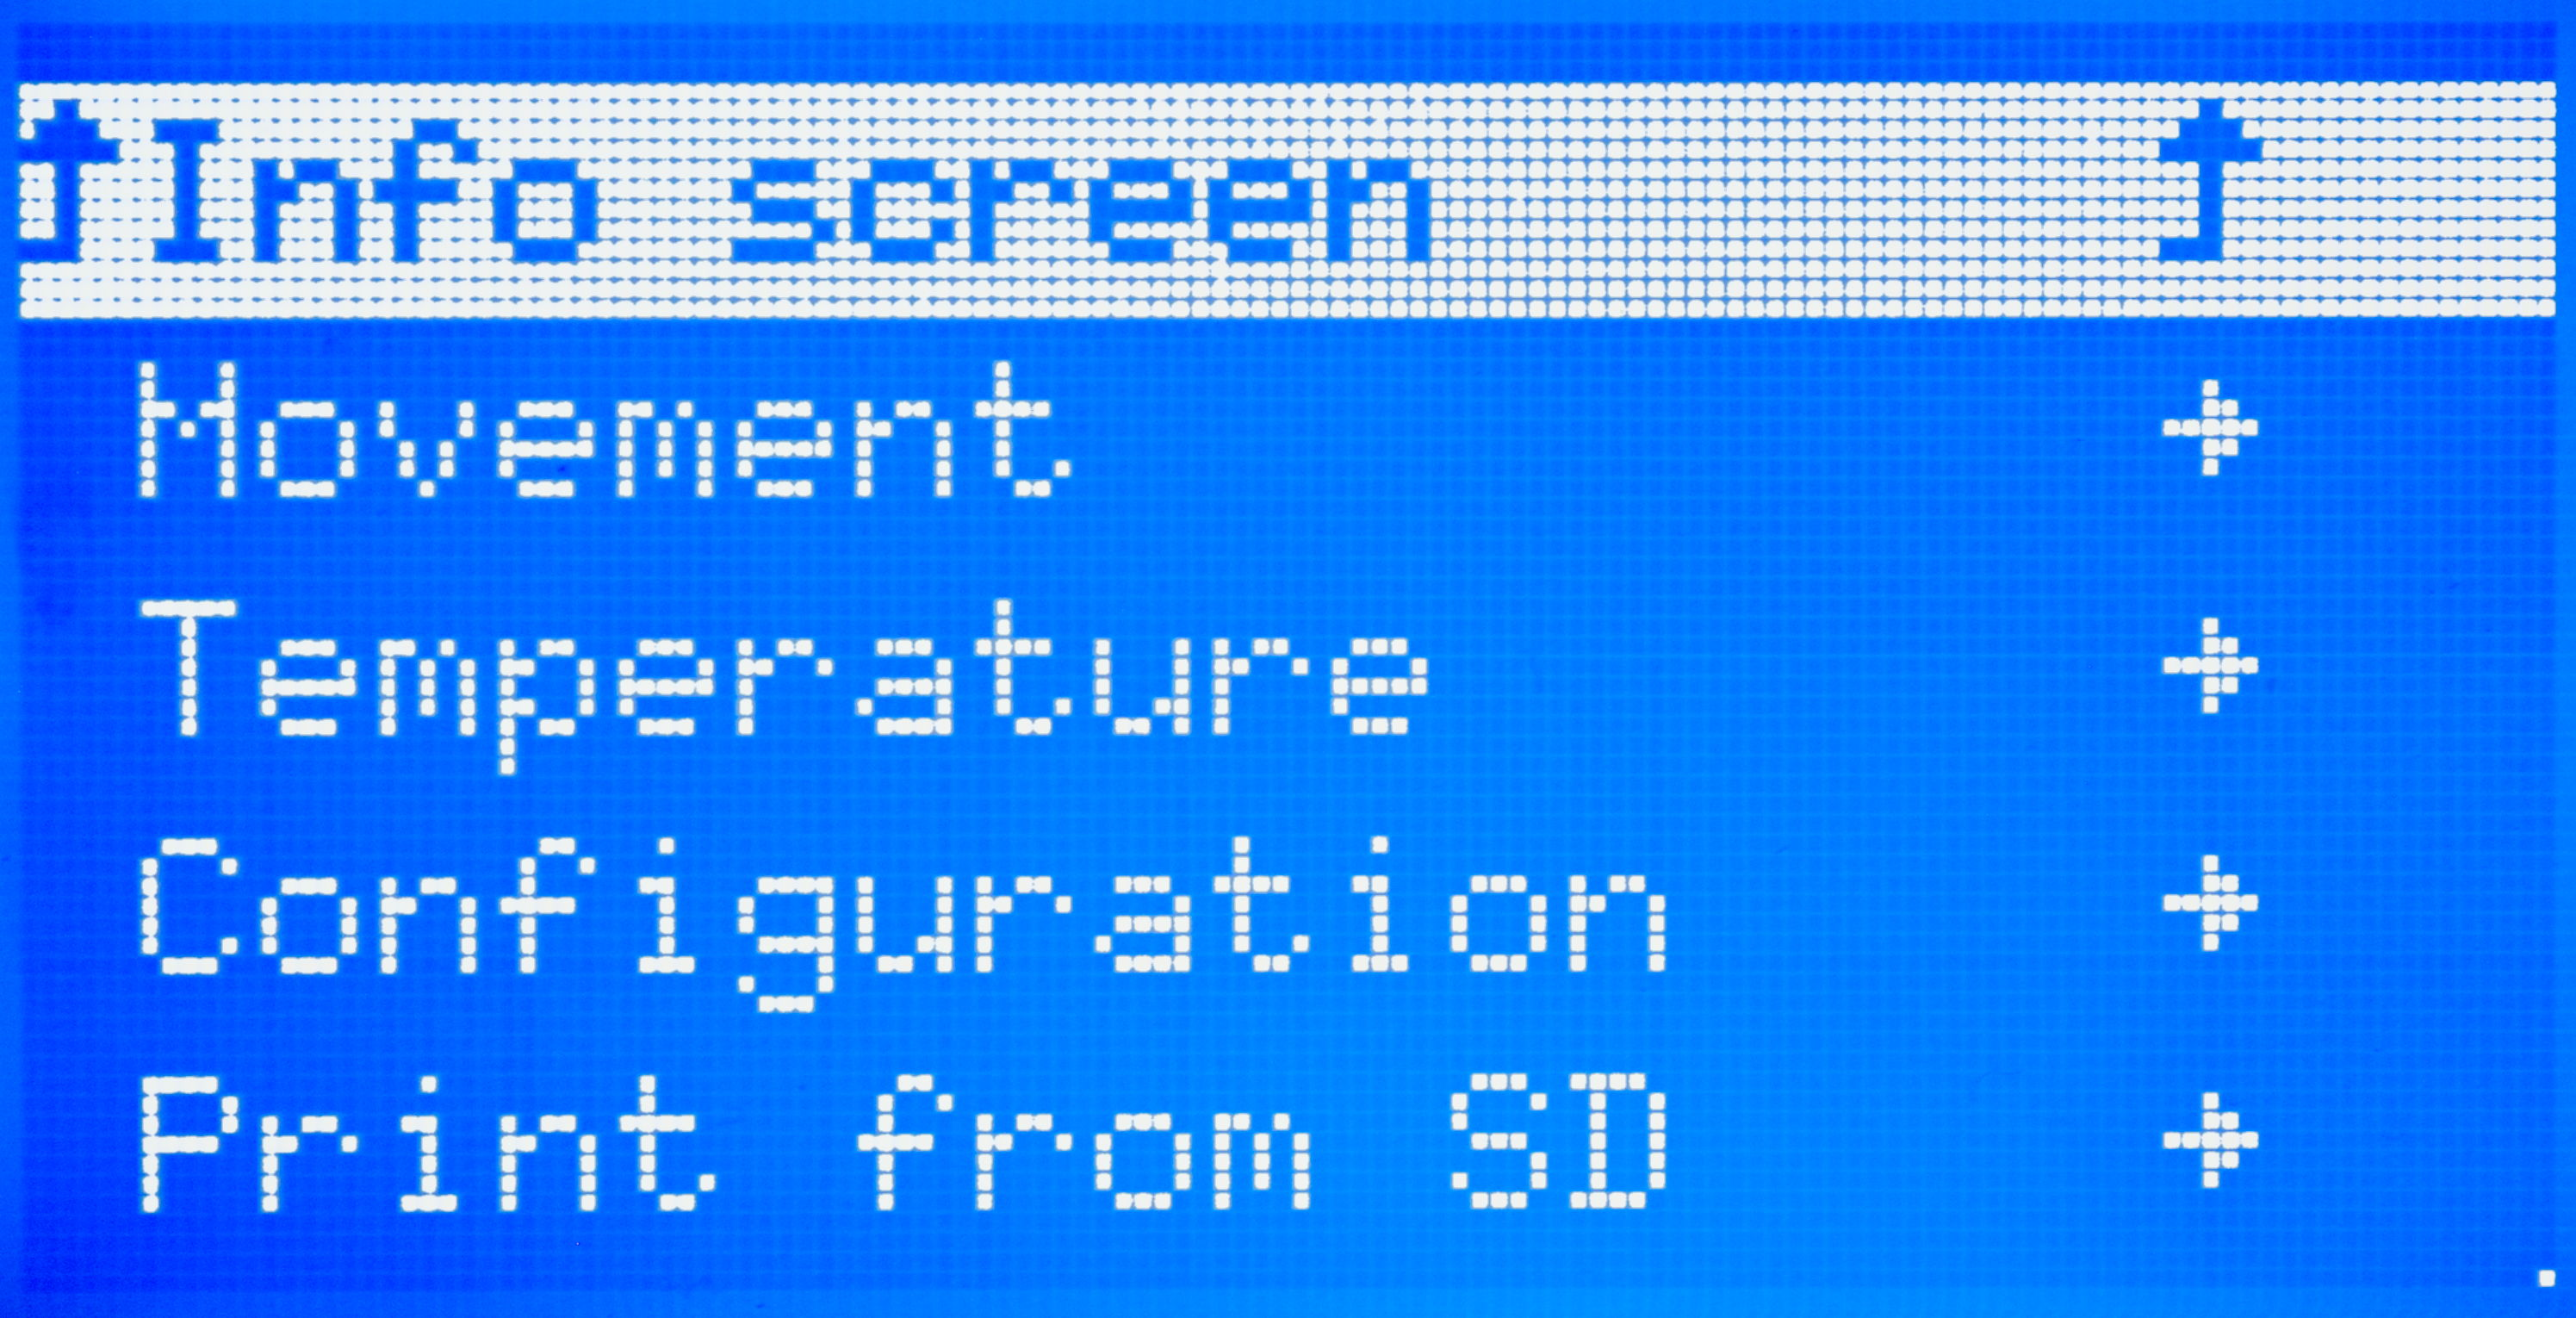
\includegraphics[keepaspectratio=true,angle=0,height=0.4\textheight,width=1.0\textwidth]{LCD_Menu.jpg}
%\caption{Main Menu}
%\label{fig:main_menu}
%\end{figure}

Out of the box, the LulzBot TAZ 3D printer is already calibrated for printing. However, the GLCD does allow tuning of the more advanced configuration settings. \textcolor{red}{We highly suggest you not modify the configuration settings unless you are certain it is necessary}. The configuration section contains settings that control how your printer operates.

\subsection{\texttt{Changing EEPROM Settings}}
\index{eeprom settings}
The \texttt{Store Memory} and \texttt{Load Memory} functions will store and load the changes you make using the GLCD Controller. You must use the \texttt{Store Memory} function to save the adjusted settings when the printer is powered on. If you ever need to revert to the original factory settings navigate to \texttt{Control} \texttt{->} \texttt{Restore Failsafe}. Clicking \texttt{Restore to Factory} will set all configuration settings back to the original factory settings in the firmware.

For more information on the configuration settings please see the LulzBot TAZ support page at \texttt{LulzBot.com/support}.

\section{\texttt{Advanced Settings}}
In the advanced settings, you can control/modify your Z offset, maximum velocity, acceleration, jerk, and esteps/mm. Once again \textcolor{red}{we highly suggest you not modify the configuration settings unless you are certain it is necessary}. Making incorrect adjustments of these settings can have adverse affects on your prints, and potentially damage your machine.

\subsection{\texttt{Z Offset}}
\index{Z Offset}
Your TAZ 6 has the ability to change the first layer height (Z offset) directly through the GLCD, even while printing the first layer. Using the GLCD, navigate to \texttt{Configuration -> Advanced Settings -> Z Offset}. While in this screen you can rotate the LCD knob counter-clockwise to bring your nozzle closer to the print surface, and rotate it clockwise to bring it farther away from the bed. Push in the LCD knob to save your settings.

\begin{figure}[H]
\centering
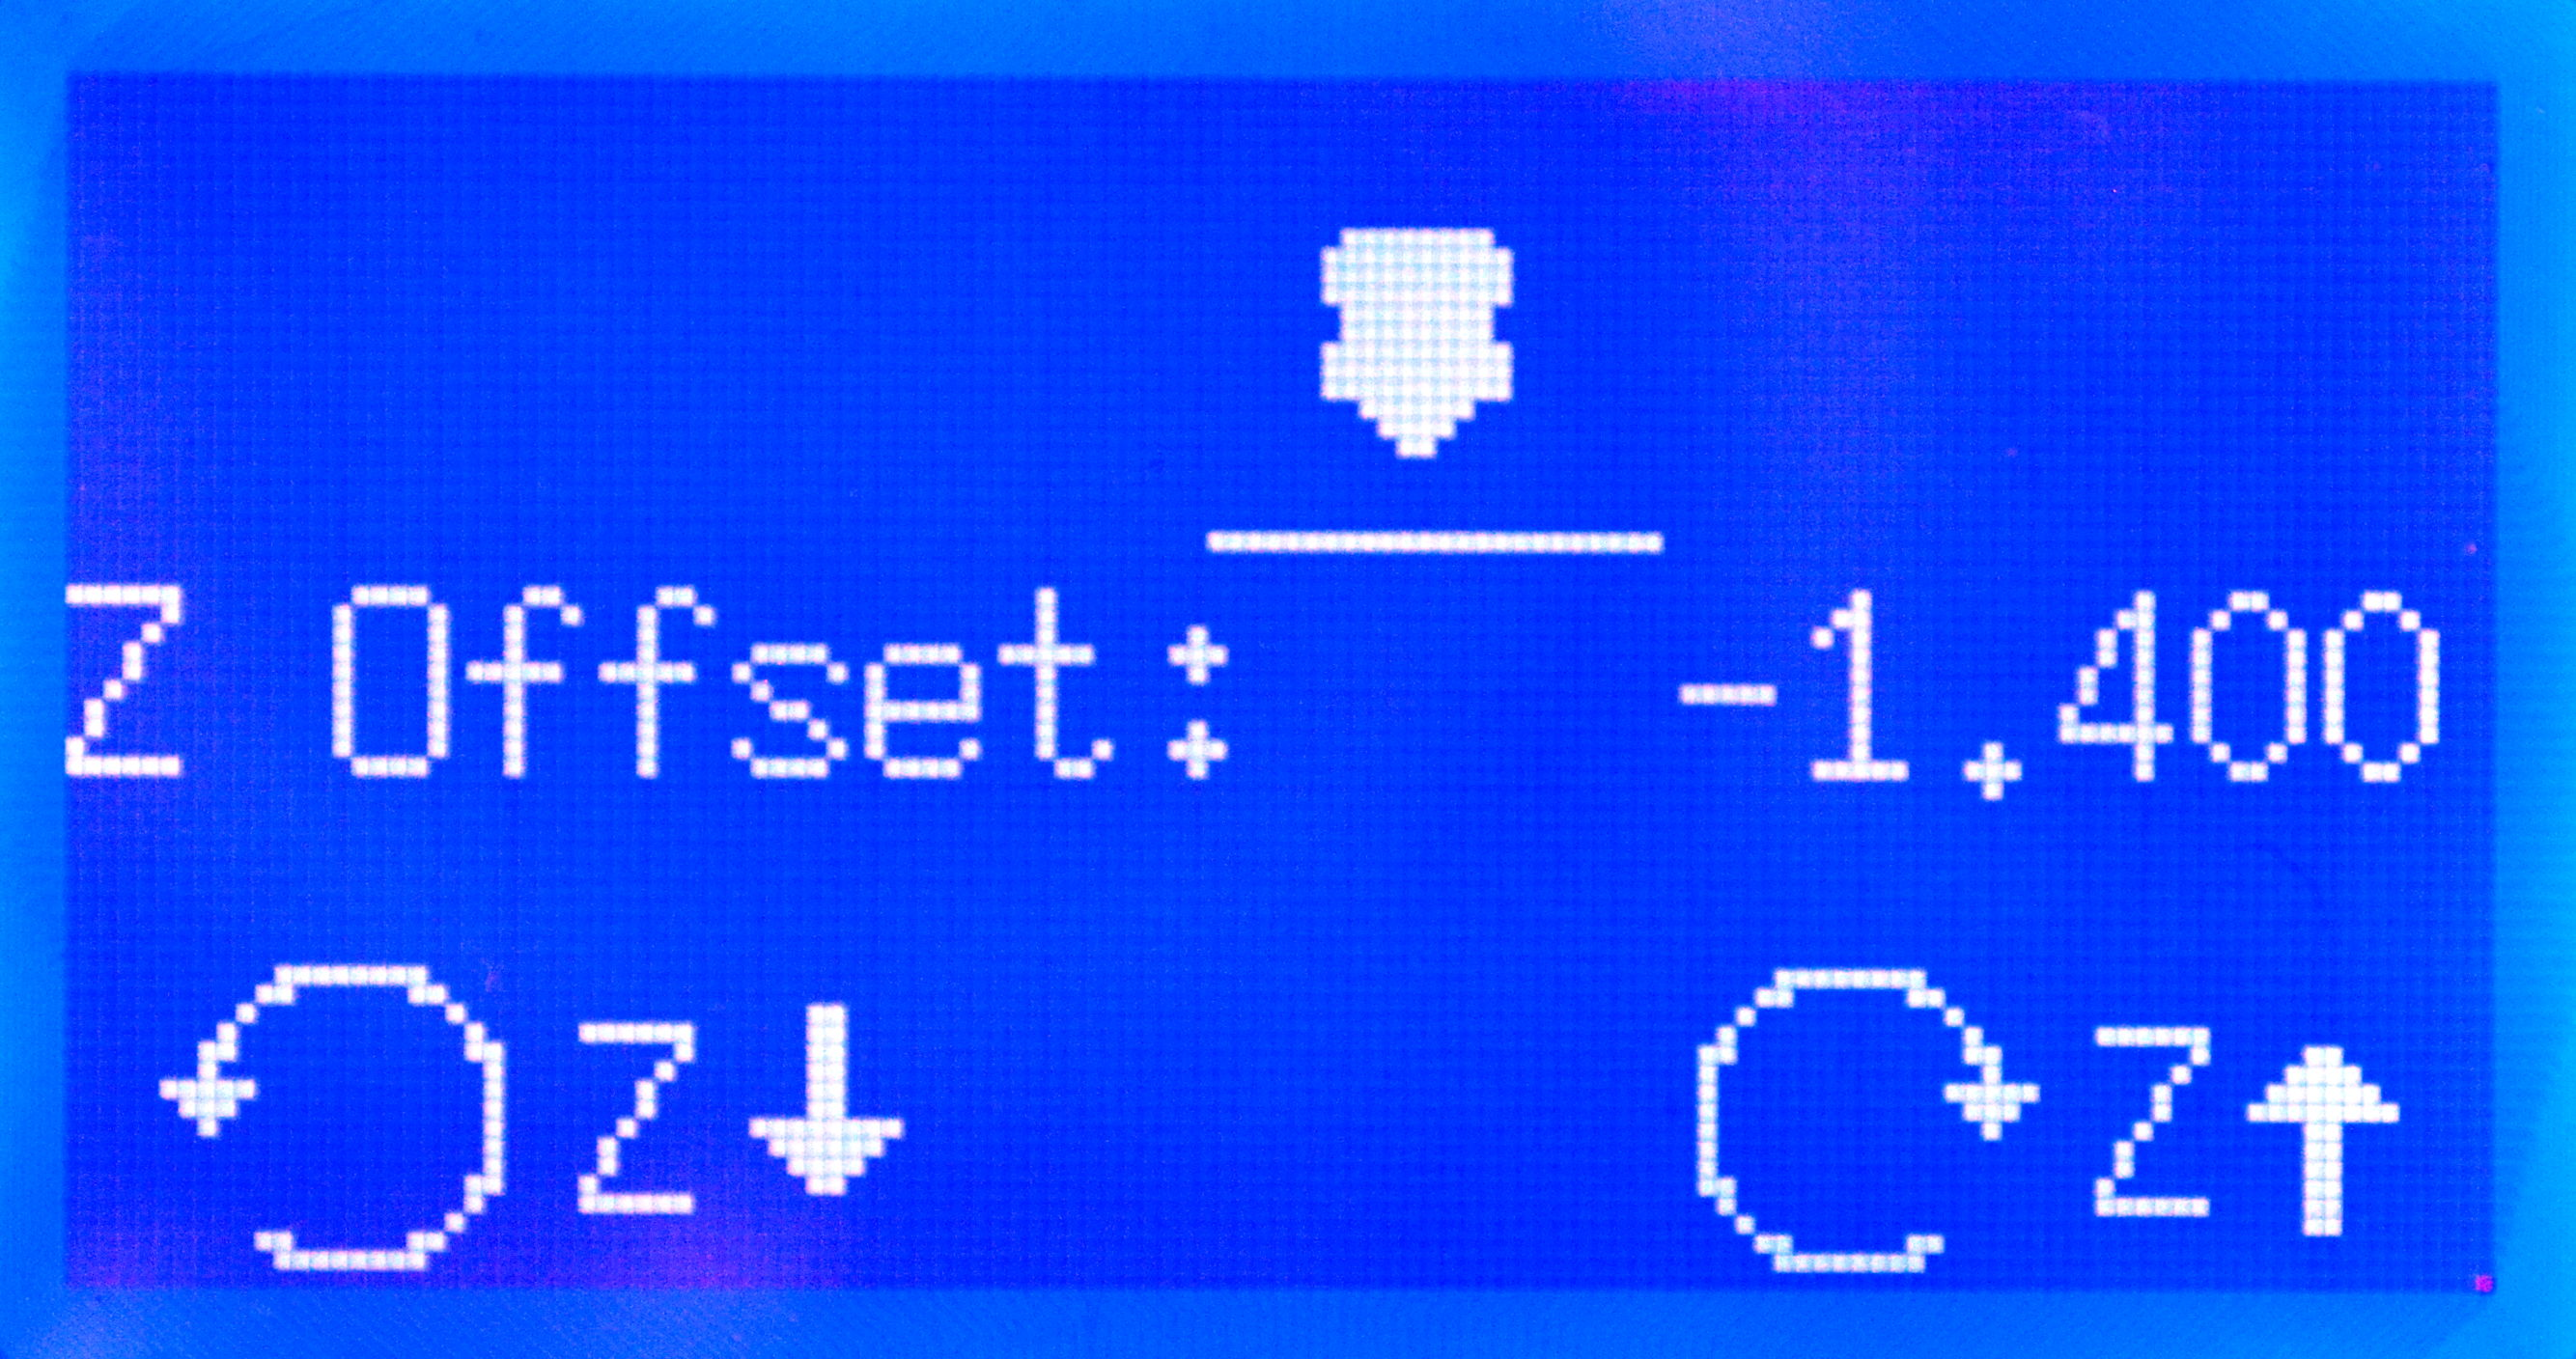
\includegraphics[keepaspectratio=true,angle=0,height=0.4\textheight,width=1.0\textwidth]{z-offset.JPG}
\caption{Z Offset Screen}
\label{fig:Z_offset_screen}
\end{figure}

%\subsection{\texttt{Change Filament}}
%While printing from SD card, you can change filament by going to \texttt{Tune -> Change Filament}. This will park your print head in the front left corner, and eject the filament from the hot end. Once you have swapped filament, go to \texttt{Tune -> Resume Print}. In order to get a crisp, clean color change you will need to manually push filament through the head until the previous color has been purged. 

%To find the configuration settings, navigate to the main menu and then select \texttt{Control} (Figure \ref{fig:configuration_menu}, page \pageref{fig:configuration_menu}). In the Control configuration settings you will find temperature and motion settings. Among others, these settings include default temperature settings and axis steps per millimeter.

\subsection{\texttt{Acceleration}}
Acceleration is the derivative of speed, and determines how quickly your print head and bed will reach defined speeds. We have this set to 500mm/s\textsuperscript{\miniscule{2}} to help prevent resonance and shadowing. This can be increased for sharper corners and faster turns, however it can lead backlash issues.

\subsection{\texttt{Jerk Settings}}
Jerk is the derivative of accleration and will determine the maximum speed change allowed at any given time. \texttt{VXY- Jerk} will control jerk setting for your X and Y axis. \texttt{VZ - Jerk} will control the jerk setting for your Z axis. \texttt{VE - Jerk} will control the jerk settings for your extruder.

\subsection{\texttt{Vmax}}
The Vmax settings will determine the maximum speed that your printer can move on any specific motor(s). We recommend leaving these settings as is. Increasing these speeds too much can lead to skipped steps and/or binding. There will be an individual section for \texttt{X, Y, Z, and Extruder} motors. 

\subsection{\texttt{Vmin}}
This sets the minimum overall speeds. We have this set to 0 by default to allow greater control through your preferred slicing program. 

\subsection{\texttt{VTrav Min}}
This will set the minimum travel speed when the tool head is not extruding. We have this set to 0 by default to allow greater control through your preferred slicing program. 

\subsection{\texttt{Amax}}
The \texttt{Amax} settings will allow you to define a maximum acceleration limit for each motor. Increasing these may reduce print time, but can result in in shadowing and resonance issues.

\subsection{\texttt{A-Retract}} 
This sets the maximum acceleration for retraction moves of the extruder. Going too high can lead to stripping, and going too low can lead to dripping. We have this set to 3000mm/s\textsuperscript{\miniscule{2}} by default.

\subsection{\texttt{Steps/mm}}
Your TAZ 6 printer will come pre calibrated on all axis for accurate movement. These settings control that movement, and if adjusted your objects will not come out at the proper dimensions. \textcolor{red}{\texttt{We only recommend adjusting your Esteps/mm}} as this can be fine tuned for individual tool heads and filaments. 

\subsection{\texttt{GLCD Controller Menu Map}}
\begin{figure}[H]
\centering
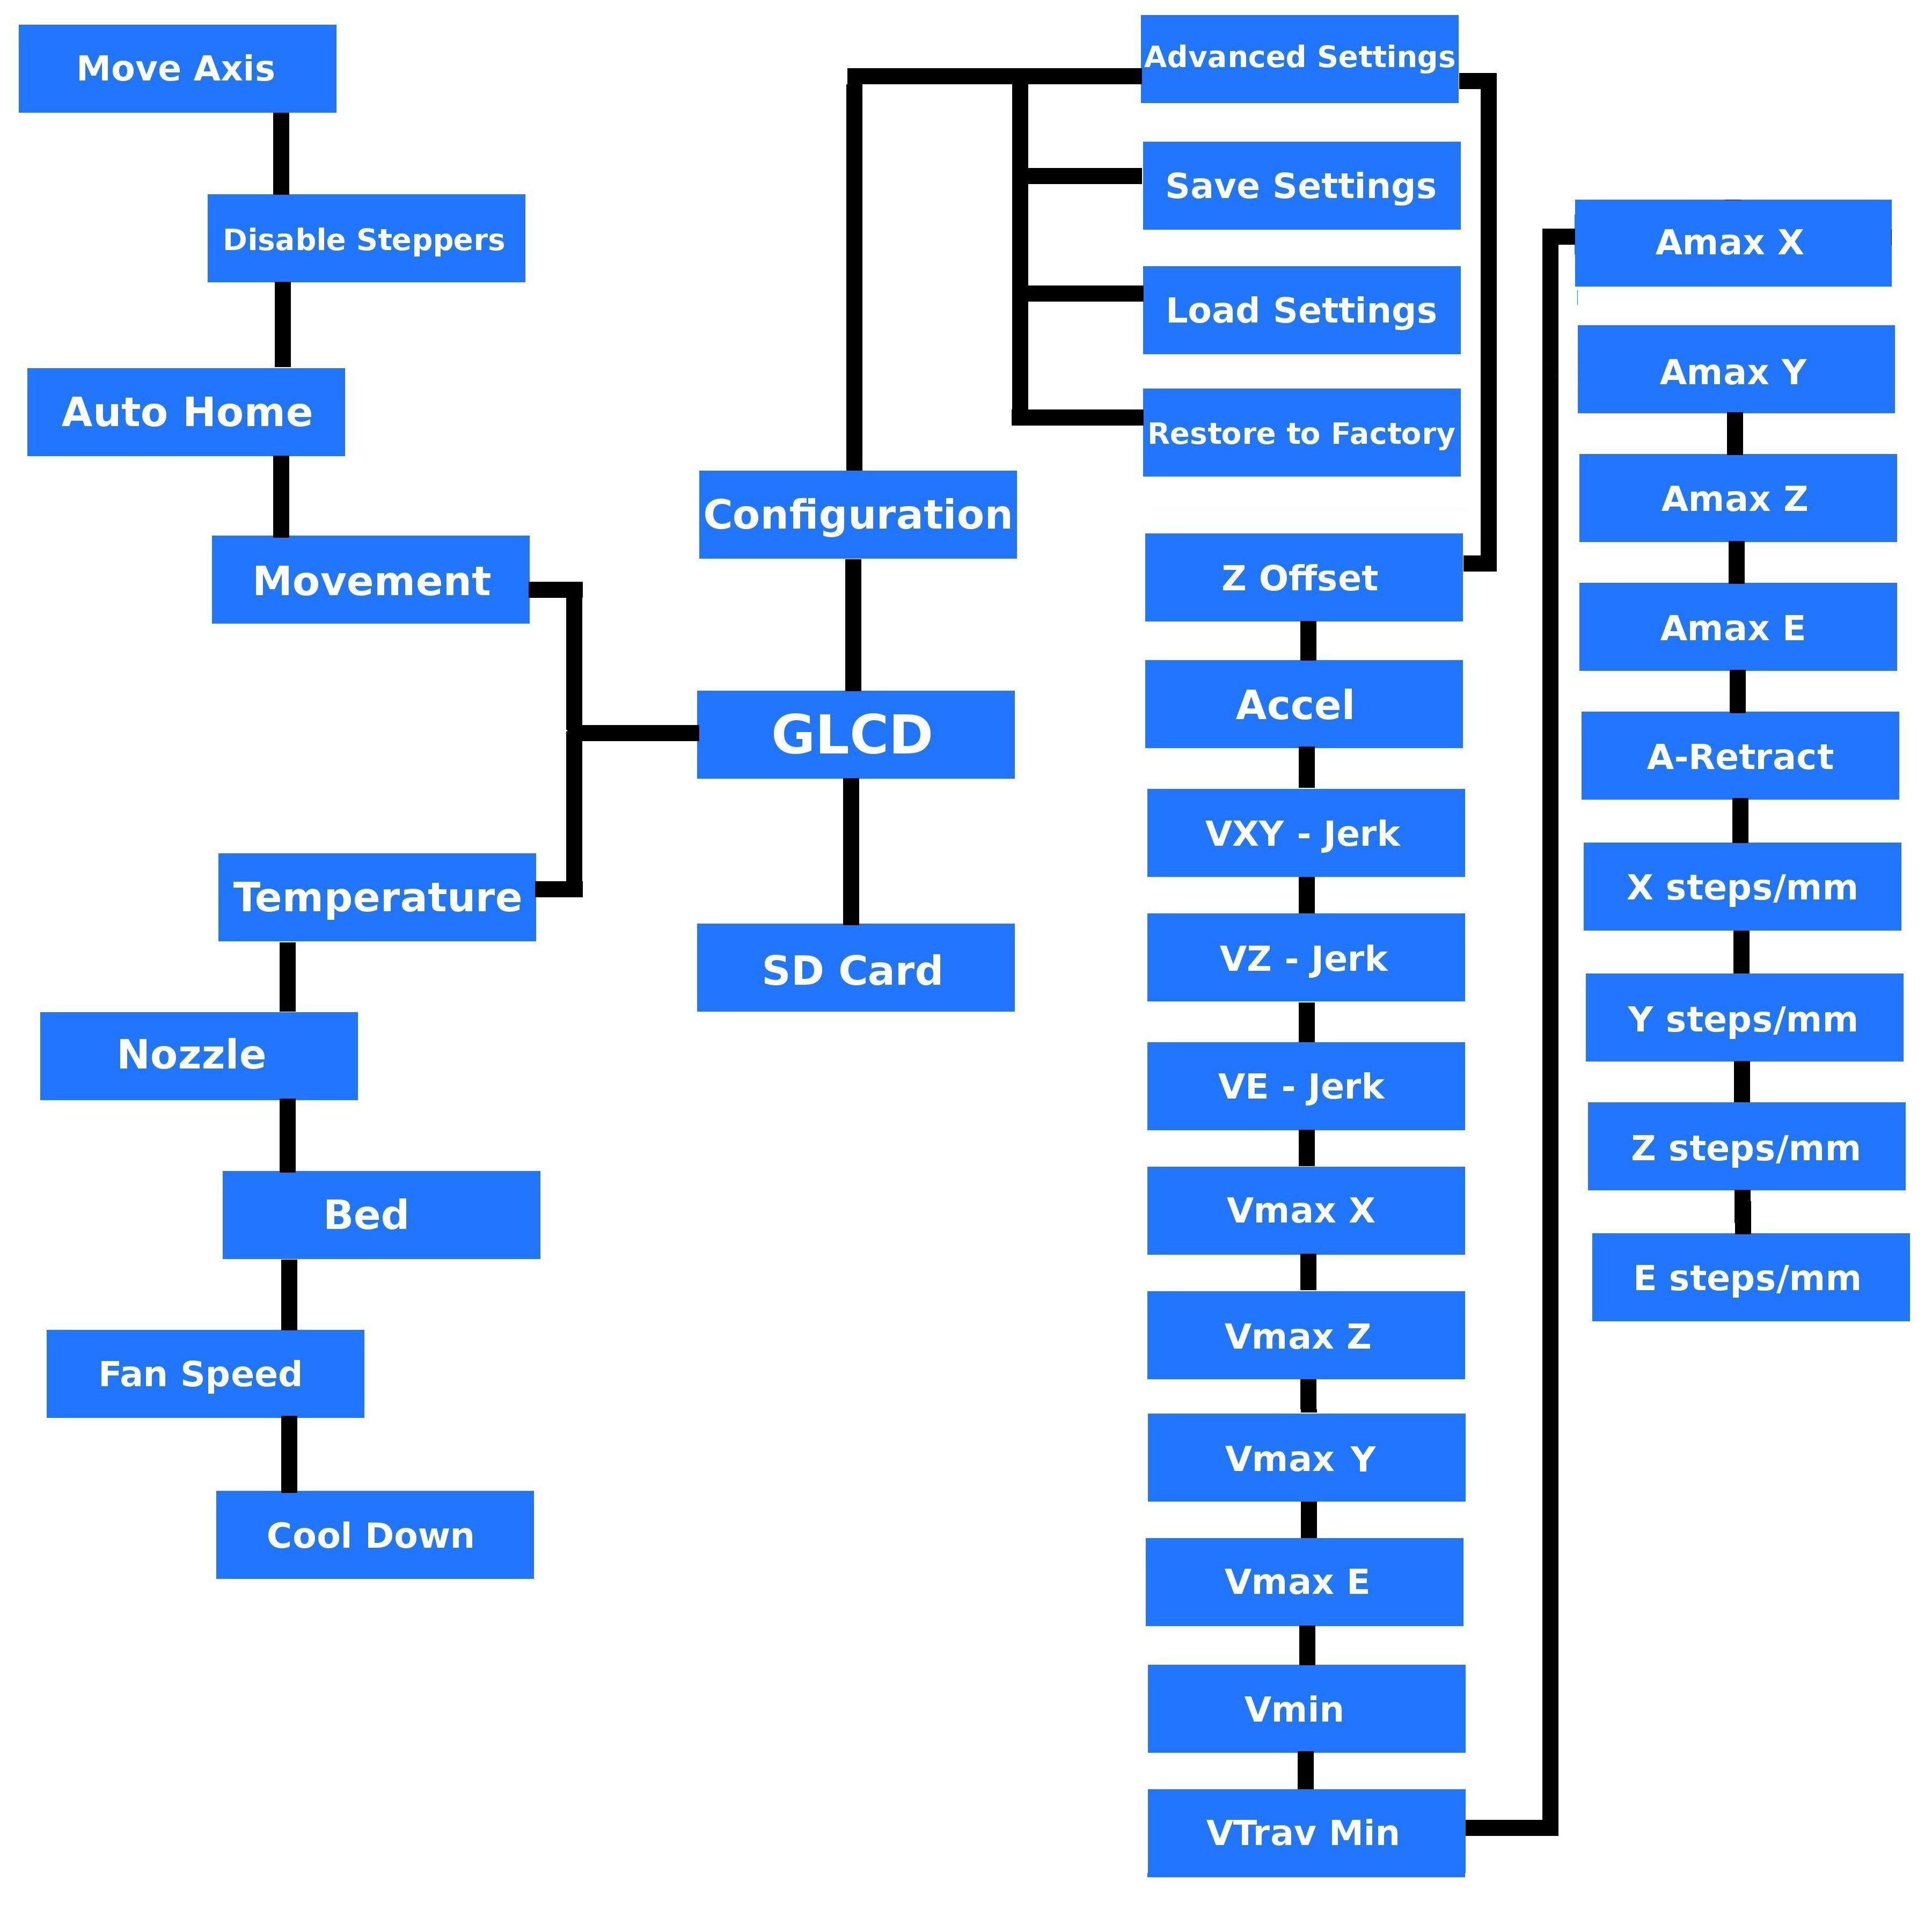
\includegraphics[keepaspectratio=true,angle=0,height=1.0\textheight,width=1.0\textwidth]{tree.jpg}
\caption{GLCD Map}
\label{fig:GLCD_Map}
\end{figure}




